\clearpage
\section{Apache ZooKeeper}
We have relied heavily on ZooKeeper in order to store our Voldemort configuration data as well as handling coordination in Headmaster. In this section we will explain what ZooKeeper is along with how it works. Finally we will present which techniques we have used along with how we used them. 

\subsection{What is ZooKeeper}
From Apache ZooKeepers own website\cite{zookeeper} they explain ZooKeeper as:

\blockquote{ZooKeeper is a centralized service for maintaining configuration information, naming, providing distributed synchronization, and providing group services. All of these kinds of services are used in some form or another by distributed applications.}

The beauty of ZooKeeper is the simplicity of the design. ZooKeeper provides a powerful service but it is up to each individual application to design how to use it. 


\subsection{Znodes}
ZooKeeper behaves almost like a file system with one key difference. Instead of files and directories - we have znodes. These znodes can contain information in the form of text. One znodes can have children which again can have more children. Together they form an hierarchical structure. 

Znodes also include version numbers for data changes, ACL changes and timestamps to allow cache validations as well as coordinate updates. Whenever a znode's data is change, it's version number increases. This is also true for whenever a client receives data. 

\begin{figure}[h]
    \centering
    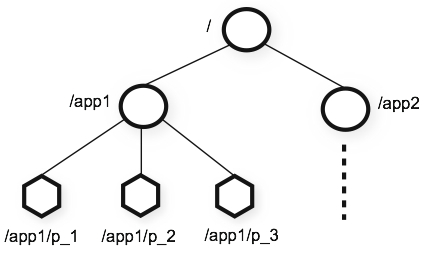
\includegraphics[width=0.4\textwidth]{software/zknamespace.jpg}
    \caption{A sample namespace}
    \label{fig:zk_namespace}
\end{figure}

These znodes can have different flags set which control their behavior. These are persistent, ephemeral and sequential. Persistent is self explanatory. When this flag is set during a put operation. The data will remain in ZooKeeper even though the client loses its connection to ZooKeeper. Ephemeral is the opposite. Data placed in ZooKeeper with this flag will be deleted when the client loses its session. If sequential is set to be true then each child of the znode will have a sequence number appended to its path. These numbers will be in strict increasing order according to which node was placed first in ZooKeeper. Ephemeral and sequential are powerful features which enable us to utilize ZooKeeper for leader election, coordination as well as locks. 


\subsection{Watches}
Watches is a 





As mentioned ZooKeeper can be used for more than just storing configuration data. In this section we will explain some different ways to use ZooKeeper.



\subsubsection{Leader election}
Leader election is something that frequently needs to be addressed in a distributed system. In our own Headmaster client we used ZooKeeper to handle this issue. 

Implementing leader election using ZooKeeper is quite straight forward. First we create a znode on some path with the sequential flag set. This ensures that each child node now will have a sequence number appended to its path. Any application wanting to act as a leader now simply creates a child znode with a predetermined name and the ephemeral flag set. This ensures that if the application becomes unavailable, the znode will be deleted.   


\subsection{implementation}
awd awd awd  adaw a daw

 
